\section{Introduction}
Let's consider the following Smart House scenario. We have $150W$ generator which is available. We know that the user comes back from work at some time defined by a gaussian distribution $N(5pm, 5m)$. Moreover we know that sun sets at time defined by $N(7pm, 1m)$. We would like to meet the following constraints with the overall probability at least $98\%$:
\begin{itemize}
\item Wash clothes (duration: $2h$, power usage: $130W$) before user comes back from work
\item Cook dinner (duration: $30m$, power usage: $100W$) ready within 15 minutes of user coming back from work
\item Have the lights on (power usage: $80W$) from before sunset to at least midnight.
\item Cook a late night snack (duration: $30m$, power usage: $20W$) between 10pm and 11pm.
\end{itemize}


\begin{figure}[H]
\begin{center}
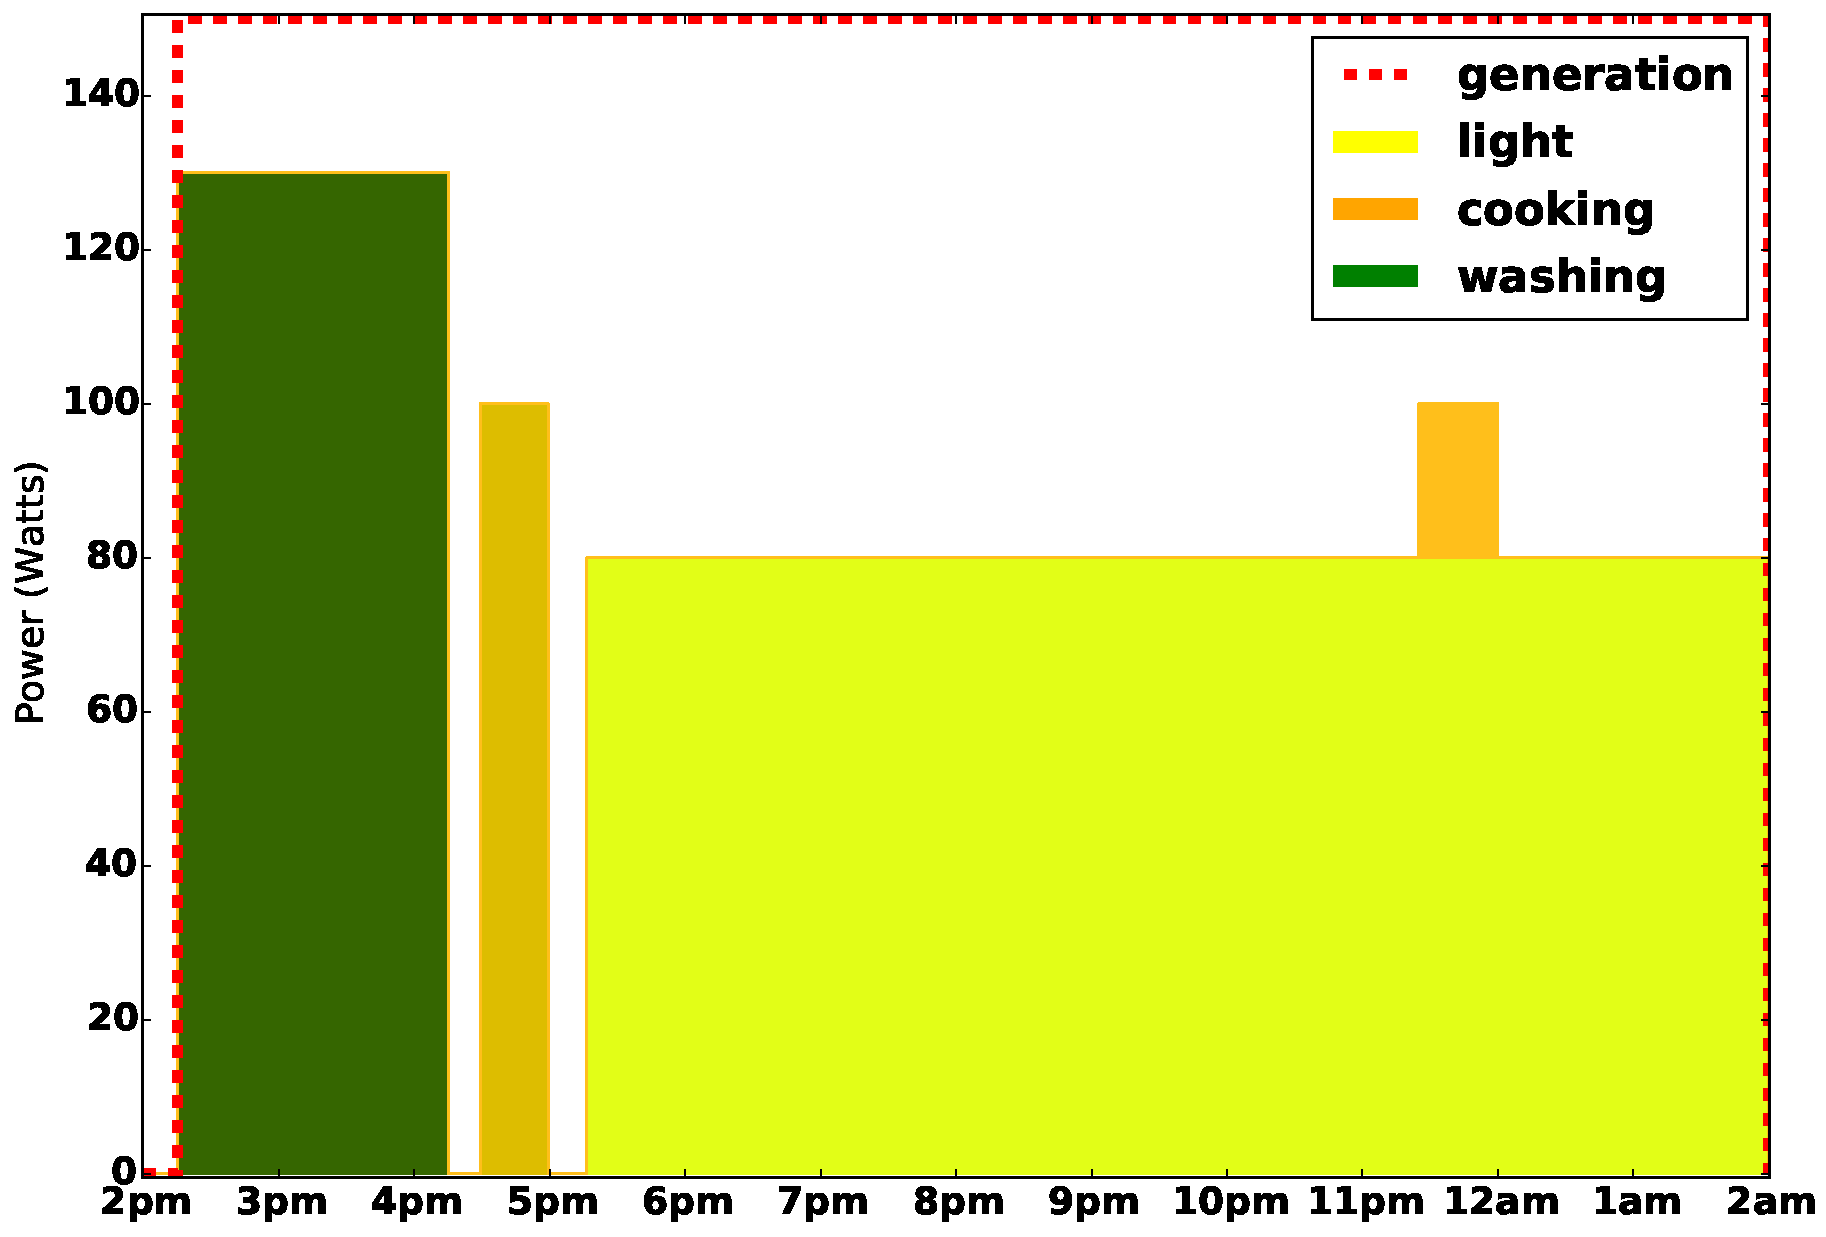
\includegraphics[width=0.49\textwidth]{pstnu_scheduling}
\caption{Depiction of solution to TRN spanning a pSTN.}
\label{fig:pstnu_scheduling}
\end{center}
\end{figure}

Our algorithm successfully finds a solution to this scenario which meets the constraints with probability $99,7\%$, which is more than required. It is presented on fig. \ref{fig:pstnu_scheduling}.
